\begin{task}{0}
Напишите какие-нибудь важные примеры оформления.
\end{task}

\begin{solution}
Некоторые варианты корректного написания многоточия: \verb'\dots', \verb'\ldots', \verb'\cdots', получается $\dots, \ldots, \cdots$. 

Смотря на предложенные примеры, обратите внимание, что везде каждое завершенное математическое выражение должно восприниматься, как отдельный член предложения. Например, если предложение оканчивается формулой, то нужно поставить точку после формулы. А если несколько завершенных выражений перечислены подряд, то между ними ставятся запятые. 

Для начала нового абзаца просто оставляйте пустую строку перед ним (или используйте команду \verb'\par'). Текст, содержащий группу формул вида $v_i\in V$, $i\in\{1,2,3\}$. 

Выключная формула, содержащая текстовое описание: 
\[F(x)=\sum_{i=0}^{n} f_i(x) \quad \text{для любого $x\in{X}$.}\]

Формула со случаями с примером применения ссылок:
\begin{equation} \label{eta_label}
\eta_{ab}=
\begin{cases}
	1, & \text{если $a\mathrel{|} b$ или $b\mathrel{|} a$,} \\
	0 & \text{иначе}.
\end{cases}
\end{equation}
Из~\eqref{eta_label} получаем требуемое.
\end{solution}

При отсутствии необходимости ссылаться на формулу ставится <<звездочка>> * (далее она в \emph{multline}), так у формулы не появится номер, а для корректирования размеров скобок используются парные команды: 
\begin{itemize} 
\item \verb'\left' и \verb'\right', 
\item \verb'\bigl' и \verb'\bigr', 
\item \verb'\Bigl' и \verb'\Bigr', 
\item \verb'\biggl' и \verb'\biggr', 
\item \verb'\Biggl' и \verb'\Biggr'.
\end{itemize} Cкобки должны быть не ниже содержимого, разве что нижние и верхние индексы можно оставлять чуть выступающими за скобки, это относится как к круглым скобкам, так и к любым другим, например, скобкам целой части или скобкам взятия модуля:
\begin{multline*}
   \left(\frac{1}{n}-\frac{1}{n+1}\right)\cdot\left\lceil\frac{3}{2}\right\rceil\cdot\biggl(\sum_{k=0}^n \binom{n}{k}-1\biggr)\cdot (1+2+\ldots+n) \\ = \frac{1}{n(n+1)}\cdot 2\cdot(2^n-1)\cdot \frac{n(n+1)}{2} = 2^n-1.
\end{multline*}
Команда  \verb'\multline' нужна для единичной завершенной формулы, не влезающей в одну строку (как на примере выше).

Для нескольких завершенных формул подойдет центрирование \verb'\gather' или какое-нибудь выравнивание, например, \verb'\align' (не надо использовать три раза подряд \verb'\[\]'):
\begin{gather*}
	S_{11}(k)=[123\ldots(k-1)k(k-1)\ldots32],\\
	S_{12}(k)=[123\ldots(k-1)kk(k-1)\ldots32],\\
	S_{22}(k)=[123\ldots(k-1)kk(k-1)\ldots321].
\end{gather*}
Обратите внимание на запятые и точки между формулами в концовке предложения выше. 

Если в ряду нумерованных формул, оформленных при помощи окружения \verb'gather', 
необходимо некоторые формулы оставить без номера, а некоторые занумеровать, то достаточно в строке этой 
формулы поместить команду \verb'\notag':
\begin{gather}
	g_1=f\vee K=x_1^{\sigma_1}\vee\dots\vee x_l^{\sigma_l}\vee\hat f\vee(x_{l+1}\mathbin{\&}\cdots\mathbin{\&}x_n),\notag \\
	g_2=f\vee\overline{x}_{l+1}=x_1^{\sigma_1}\vee\dots\vee x_l^{\sigma_l}\vee\overline{x}_{l+1}\vee\hat f \label{eq-gather},
\end{gather}
пронумеровали формулу~\eqref{eq-gather}.

В \emph{align} применяются \& для определения позиций выравнивания:
\begin{align*}
1 &= 10^0, \\
11 &= 10^0+10^1, \\
111 &= 10^0+10^1+10^2.
\end{align*}

Оформление теорем, доказательств, подпунктов доказательства (нумерованные списки), осуществляется так (окружения theorem, lemma, proposition заданы в файле main).

\begin{proposition}\label{остов в уницграфе}
В унициклическом графе всегда можно выделить не менее трех различных остовных деревьев.
\end{proposition}
\begin{proof}
В унициклическом графе имеется простой цикл длины $k\geqslant 3$. Поскольку граф по определению является связным, удалив из него любое из $k$ ребер цикла, получим остовное дерево, причем удаление разных ребер приводит в итоге к разным остовным деревьям. Таким образом, в графе найдено $k\geqslant 3$ различных остовных деревьев.
\end{proof}

Далее пример применения ссылки на утверждение (слово <<утверждение>> при этом опускать нельзя). 

\begin{lemma}
Утверждение леммы, можно с формулой: 
\[ a  + b = c.\]
\end{lemma}
\begin{proof}[Доказательство]
Проведём индукцией по $n$. Применим утверждение~\ref{остов в уницграфе}. Текст. 
\end{proof}

Далее обратите внимание также на возможность сослаться на конкретный пункт доказательства с использованием \verb'\label{}' и \verb'\ref{}'.

\begin{theorem} [критерий Эрдёша\,--\,Галлаи] \label{degree_seq_rlz}
    Последовательность $d_1\geqslant d_2 \geqslant \dots \geqslant d_n,$ состоящая из  $n\geqslant 2$ неотрицательных целых чисел, реализуема некоторым графом тогда и только тогда, когда $\sum_{i=1}^n d_i$~--- чётное число и при этом выполнено:
    \[
        \sum_{i=1}^t d_i \leqslant t(t-1) + \sum_{i=t+1}^n \min\{t, d_i\} \quad \forall \; 1 \leqslant t \leqslant n-1.
    \]
\end{theorem}
\begin{proof}
Разберем несколько случаев: 
\begin{enumerate}
    \item Пусть выполняется $X$.
    \item Пусть выполняется $Y$. Возможны следующие случаи.
    \begin{enumerate} 
        \item \label{a+b=10} Случай $a+b=10.$ 
        \item Случай $a+b=11.$ 
    \end{enumerate}
    \item Случай $a+b=12.$ Данный случай аналогичен случаю~\ref{a+b=10}.
\end{enumerate}
\end{proof}

Рисунки вставляются при помощи окружения \verb'figure'. Внутрь этого окружения необходимо 
поместить команду \verb'\includegraphics{}', аргументом которой служит имя файла с рисунком (путь Fall/img/ уже заявлен для картинок в main при подключении пакета \verb'\usepackage{graphicx}'), также можно отрегулировать масштаб. 
Команда \verb'\centering' нужна для центрирования рисунка. Чтобы рисунок никуда не уплыл, в параметр позиционирования пишется [H] (параметр [H] не работал бы без подключения пакета float в main, но он уже включен в вашем проекте).

\begin{figure}[H]
\centering
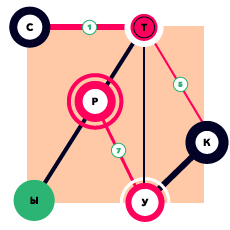
\includegraphics[scale=0.5]{Дискретные структуры картинка.png}
\caption{Эмблема дискретных структур.} \label{эмблема ДС}
\end{figure}

На рис.~\ref{эмблема ДС} можно ссылаться. 

Подрисунки можно добавлять с использованием subfigure, но для того, чтобы это окружение работало, в main надо кроме прочего добавить subcaption. Обратите внимание: несмотря на то, что вставлена фотография, контраста с белым фоном нет. Вам при фотографировании также нужно озаботиться тем, чтобы он не возникал (фотографировать сканером, а не стандартно).
\begin{figure}[H]
\centering
\begin{subfigure}[b]{0.45\linewidth}
\centering
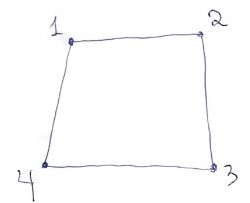
\includegraphics[scale=0.6]{Fall/img/Cycle-1.png}
\caption{Первый цикл} \label{цикл-1}
  \end{subfigure} 
  \begin{subfigure}[b]{0.45\linewidth} 
  \centering
  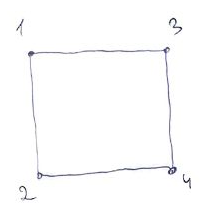
\includegraphics[scale=0.6]{Fall/img/Cycle-2.png}
  \caption{Второй цикл} \label{цикл-2}
  \end{subfigure}
 \caption{Два различных цикла.} \label{delta gamma = 2}
\end{figure}

На рис.~\ref{цикл-1} и~\ref{цикл-2} изображены два различных цикла.

Пример таблицы. Окружение \verb'array' необходимо заключать в пару \verb'$..$' для математических формул.
\begin{table}[H]
\centering
$
\begin{array}{|c|c|c|c|c|c|}
	\hline
	\text{Формула} & (1) & (2) & (3) & (4) & (13)\\
	\hline
	\exp\Gamma(\varphi^T) & 123202 & 702 & 4202 & 702 & 16\\
	\hline
\end{array}
$
\caption{Формула.} \label{таблица с формулой}
\end{table}
    


